\documentclass[8pt]{beamer}

\usepackage[T1]{fontenc}
\usepackage[polish]{babel}
\usepackage{booktabs}
\usepackage{multirow}
\usepackage[table]{xcolor}
\usepackage{amsmath}
\usepackage{graphicx}
\usepackage{float}
\usepackage{polski}
\usetheme{berlin}

\title{Projekt Analiza Sygnałów}
\subtitle{Mierzenie pojemności kondensatora}
\author{Teodor Dimitriadis, Sonia Mituś, Robert Włodkowski}
\date{15 czerwca 2026}

\begin{document}
\begin{frame}
\titlepage
\end{frame}
%wstęp
\begin{frame}{Wstęp}
Proces ładowania i rozładowania kondensatora rozpoczyna się od podpięcia pustego kondensatora do obwodu. Na początku płynie maksymalny prąd. Następnie elektrony zaczynają ładować kondensator, rośnie na nim napięcie. W rezultacie w obwodzie zaczyna spadać natężenie. Kiedy napięcie kondensatora będzie takie samo jak napięcie zasilania, jest on maksymalnie naładowany, prąd przestanie płynąć. Następnie rozpocznie się proces odwrotny, rozładowywanie. Elektrony zgromadzone w kondensatorze zaczną płynąć, ale w przeciwnym kierunku niż wcześniej. Z czasem spadają napięcie i natężenie, aż osiągną zero. Kondensator jest całkowicie rozładowany. Ten proces się powtarza.
\end{frame}
\begin{frame}{Wstęp}{Równania Różniczkowe}
Z równań różniczkowych (rozpisane niżej) wynika zależność $Q(t) = ECe^{\frac{-t}{RC}}$. W rzeczywistej realizacji oznacza to, że kondensator potrzebuje czasu, aby napięcie się zmieniło. Opiera się on nagłym, intensywnym zmianom.
\end{frame}
\begin{frame}{Wstęp}{Powód przeprowadzenia badania}
W zależności od wyboru $\alpha$ oraz $\beta$, czyli parametrów naładowania, wyniki były różne. Dla niektórych parametrów wartości pokrywały się z modelem matematycznym, a dla innych nie.
\end{frame}

%Teoria
\begin{frame}{Opis Teoretyczny}{Ogólna teoria}
    Założeniami modelu jest fakt, że jest on izolowany oraz dostarczane jest idealne źródło napięcia - E. W kondensatorze energia gromadzona jest w postaci pola elektrycznego. Składa się on z dwóch przewodzących elektrod rozdzielonych dielektrykiem. Zjawisko gromadzenia ładunku elektrycznego opisuje definicja pojemności:
	$$ C = \frac{Q}{U_c}$$
	gdzie $Q$ to ładunek elektryczny, a $U_c$ to napięcie na kondensatorze.
	
\end{frame}
\begin{frame}{Opis Teoretyczny}{Ogólna teoria}
    Z drugiego prawa Kirchoffa wiemy, że na zamkniętym obwodzie zawierającym rezystor oraz kondensator:
	$$ E = U_R + U_c$$
	gdzie $U_R$ to napięcie na rezystorze.
 Z prawa Ohma natomiast wiemy, że:
	$$ U_R = I \cdot R $$
	gdzie $I$ to natężenie prądu elektrycznego, $R$ to rezystancja oraz że:
	$$ I = \frac{dQ}{dt}$$
\end{frame}
\begin{frame}{Opis Teoretyczny}{Wzór na czas ładowania}
Rozpisując prawo Kirchoffa:
	\begin{align*}
		U_R + U_c &= E \\
		I \cdot R + \frac{Q}{C} &= E \\
		\frac{dQ}{dt} \cdot R + \frac{Q}{C} &= E \\
		R \cdot Q' + \frac{1}{C} \cdot Q &= E \\
		Q' + \frac{1}{RC} \cdot Q &= \frac{E}{R} \\
		e^{\frac{t}{RC}}Q' + e^{\frac{t}{RC}}\frac{1}{RC} \cdot Q &= e^{\frac{t}{RC}}\frac{E}{R} \\
		(e^{\frac{t}{RC}} \cdot Q)' &= \frac{E}{R} e^{\frac{t}{RC}} \\
		e^{\frac{t}{RC}} \cdot Q &= \frac{E}{R} \cdot RC e^{\frac{t}{RC}} + A\\
		Q(t) &= EC + Ae^{-\frac{t}{RC}} 
	\end{align*}
\end{frame}
\begin{frame}{Opis Teoretyczny}{Wzór na czas ładowania}
Podstawiając warunek początkowy $U_c(0) = 0 \implies Q(0) = 0$:
	$$Q(t) = EC(1-e^{\frac{-t}{RC}})$$ 
	Z tego równania wynika, że czas ładowania wynosi:
	$$t = RC \ln(\frac{E}{E - U_c}) = - RC \ln(1 - \frac{U_c}{E})$$
\end{frame}
\begin{frame}{Opis Teoretyczny}{Rozładowywanie kondensatora}
Rozpisując prawo Kirchoffa dla E=0:
	\begin{align*}
		U_r + U_c &= 0 \\
		R \cdot \frac{dQ}{dt} + \frac{1}{C} \cdot Q &= 0 \\
		\frac{1}{Q} \cdot \frac{dQ}{dt} &= \frac{-1}{RC} \\
		\int \frac{1}{Q} dQ &= -\frac{1}{RC} \int dt \\
		\ln Q &= -\frac{t}{RC} + A \\
		Q(t) &= Be^{\frac{-t}{RC}} \\		
	\end{align*}
\end{frame}
\begin{frame}{Opis Teoretyczny}{Wzór na czas ładowania}
Podstawiając warunek początkowy $U_c(0) = E \implies Q(0) = EC$:
	$$Q(t) = ECe^{\frac{-t}{RC}}$$
	Z tego równania wynika, że czas rozładowania wynosi:
	$$t = RC \ln(\frac{E}{U_c}) $$
	Wiemy więc, że pojemność kondensatora wynosi:
	$$C = \dfrac{t}{R \ln(\frac{E}{U_C})}$$
\end{frame}
\begin{frame}{Opis Teoretyczny}{Porównanie z oscyloskopem}
    \begin{figure}[H]
    \centering
    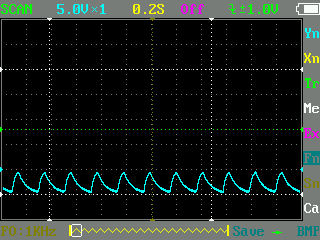
\includegraphics[width=0.9\textwidth]{wyniki/IMG_001.png}
    \end{figure}
\end{frame}
\begin{frame}{Opis Teoretyczny}{Wyznaczanie pojemności kondensatora}
Pojemnośc kondensatora będziemy mierzyć od pewnego parametru naładowania $\alpha$ do pewnego parametru naładowania $\beta$.
Koniecznym założeniem jest, aby $\alpha$ i $\beta$ były dodatnie, mniejsze od 1, oraz spełniały $\alpha < \beta$.
Wtedy $\Delta t$ będziemy nazywać różnicę czasu $t_{\beta}$ - $t_{\alpha}$ 
\end{frame}
\begin{frame}{Opis Teoretyczny}{Wyznaczanie pojemności kondensatora}
\begin{align*}
t_{\beta} - t_{\alpha} &= -RC \ln(1 - \beta) + RC \ln (1 - \alpha) = RC\ln(\dfrac{1 - \alpha}{1 - \beta})\\
\end{align*}
$$C = \dfrac{\Delta t}{R \ln(\frac{1 - \alpha}{1 - \beta})}$$
\end{frame}
\begin{frame}{Metoda Przeprowadzenia Badań}{Kwantyzacja}
    Arduino Uno ma przetwornik o 10 bitach, co przekłada się na możliwość mierzenia napięcia na zakresie 1024 poziomów, każdy z nich jest oznaczany przez liczbę od 0 do 1023. Napięcie odniesienia wynosi 5V. Tak więc jeden krok kwantyzacji wynosi 5V/1024. Przybliża się do najbliższego poziomu, więc maksymalnie możemy się pomylić o połowę tej wartości.
\end{frame}
\begin{frame}{Metoda Przeprowadzenia Badań}{Próbkowanie}
Mikrokontroler Arduino UNO potrzebuje 100 mikrosekund na wykonanie pełnego pomiaru, a teoretyczna maksymalna częstotliwość próbkowania to około 10kHz.
\end{frame}

\begin{frame}{Opis sprzętu}
Opornik ma wartość nominalną 220$\Omega$ z tolerancją $\pm2,2\Omega$. Kondensator ma nominalną pojemność $100\mu F$. Napięcie znamionowe wynosci 35V.
\end{frame}

\begin{frame}{Opis układu RC}
Układ składa się z 2 oporników, kondensatora oraz Arduino. Arduino mierzy spadki napięcia na kondensatorze. Aktywny układ korzysta tylko z jednego opornika, ponieważ drugi jest odłączony przez źródło napięcia.
\end{frame}

\begin{frame}{Wyniki}
Sporządziliśmy pomiary dla następujących par parametrów $\alpha$ i $\beta$: 0,1 i 0,9; 0,2 i 0,8; 0,3 i 0,7. Zapisaliśmy po 10 wyników dla każdej z nich. Z prawa wielkich liczb, gdy danych jest dużo ich średnia będzie w przybliżeniu zgadzać się z wartością prawdziwą.
\end{frame}
\begin{frame}{Przedstawienie wyników}
\begin{table}[H]
  \centering
  \footnotesize
  \caption{Wyniki dla różnych parametrów}
    \begin{tabular}{|r|r|r|r|}
    \toprule
    \multicolumn{1}{|l|}{$\alpha, \beta$} & \multicolumn{1}{l|}{0,1 i 0,9} & \multicolumn{1}{l|}{0,2 i 0,8} & \multicolumn{1}{l|}{0,3 i 0,7} \\
    \midrule
    1.    & 106,94 & 101,26 & 98,49 \\
    \midrule
    2.    & 107,19 & 101,26 & 99,14 \\
    \midrule
    3.    & 107,19 & 100,9 & 98,49 \\
    \midrule
    4.    & 107,21 & 100,9 & 99,14 \\
    \midrule
    5.    & 107,18 & 101,26 & 98,49 \\
    \midrule
    6.    & 106,93 & 101,26 & 99,14 \\
    \midrule
    7.    & 107,19 & 101,26 & 99,14 \\
    \midrule
    8.    & 107,19 & 101,26 & 98,49 \\
    \midrule
    9.    & 106,94 & 101,26 & 99,14 \\
    \midrule
    10.   & 107,19 & 100,9 & 98,49 \\
    \midrule
    średnia    & 107,12 & 101,15 & 98,82 \\
    \midrule
    odch. stand   & 0,01368 & 0,02722 & 0,10563 \\
    \midrule
    minimum   & 106,93 & 100,90 & 98,49 \\
    \midrule
    maksimum   & 107,21 & 101,26 & 99,14 \\
    \bottomrule
    \end{tabular}%
  \label{tab:addlabel}%
\end{table}
\end{frame}

\begin{frame}{Niepewności}
\begin{table}[H]
\centering
\caption{Niepewności}
\begin{tabular}{|l|r|r|r|}
\toprule
$u_a$    & 0,03903 & 0,05499 & 0,10835 \\
\midrule
$u_b$    & 0,61898 & 0,58462 & 0,57239 \\
\midrule
$u_c$    & 0,62021 & 0,58721 & 0,58255 \\
\midrule
$2u_c$   & 1,24041 & 1,17441 & 1,1651 \\
\bottomrule
\end{tabular}
\end{table}
\end{frame}

\begin{frame}{Analiza}
Uzyskane wyniki wskazują, że wyznaczona pojemność kondensatora znajduję się w zakresie tolerancji wartości nominalnej $100 \mu F$ w dwóch z trzech analizowanych przypadków.
Rozbieżność w pierwszym wariancie spowodowana może być z wykładniczego charakteru krzywej ładowania, gwałtownego wzrostu na początku, oraz znaczącego zwolnienia przy końcu. Dobranie parametrów $\alpha = 0.2$ oraz $\beta = 0.8$ pozwoliło na wyelminowanie zniekształceń pomiarów.
\end{frame}
\end{document}